This section introduces an extension of the asynchronous calculus for timed processes~\cite{Bocchi2019}, catered for the new Timeout Session Types.

In definition that follows
\begin{inline}
   \item \epointp\ and \epointq\ are two endpoints
   %
   \item \pchan\ is a channel between two endpoints
   %
   \item \pchan\ is a channel between two endpoints
   %
   \item \bool\ is a boolean condition
   %
\end{inline}
\pbuffer\ is an ordered sequence of messages, functioning either as: a channel buffer; or, a list of messages to discard.
\prequeue\ is a sequence of messages waiting to be received, with branches added dynamically at run-time, and facilitates a process recalling to an earlier point and taking a different branch.
\precallcache\ is each an ordered list of the messages sent corresponding to each of the receiving branches able to trigger a recall; this is used to ensure that there are no messages left in the queue that are unable to be received.

The process variable \prcvar\ contains the following ordered sequences
\begin{inline}
   \item \setLabel\ of message labels
   %
   \item \setChan\ of session channels
   %
\end{inline}
\begin{equation*}
   \mproccescalc%
\end{equation*}
The following sections provide an in-depth description on the possible forms a process can take, with a focus on the new additions. Specific details and design decisions become clear when considered in the context of the reduction steps, shown later in~\cref{ssec:prc_reduction_rules}.

\subsubsection*{Sending Messages}\hfill\mbox{$\mpsendalways$}\mbox{ }\par%
As standard, a process \prc\ can send a message \msglabel\ on channel \pchan\ and continue as \qrc.
Sending actions such as these can now be accompanied by a set of branching receiving actions.

\paragraph*{Listening for Timeouts}\hfill\mbox{$\mpsendlisten$}\mbox{ }\par%
In additional to performing standard sending actions, a process can provide a set of messages that can potentially be received after this sending action, within $n$ time units, and pertain to a different viable branch.

These potential receptions are moved to a \emph{listener} process private to the sending individual, and is able to continue listen for, and receive, those messages arriving in the queue once the main thread has progressed onwards.

\subsubsection*{Listeners}\hfill\mbox{$\mprcrecall$}\mbox{ }\par%
A \emph{listener process} is a private to an individual, and runs in parallel to the main thread.
Messages accumulated by the listener correspond to the entry points to other branches this process could have possibly taken, in the case that the other participant has unknowingly taken one of these branches.

\paragraph*{Tidying Messages}\hfill\mbox{$\mathtt{tidy}:\mpbuffer$}\mbox{ }\par%
A listener process is always able to receive a special \texttt{tidy} message, which contains an ordered sequence of messages to be ignored from their queue.

\paragraph*{Message Logs}\hfill\mbox{$\mkset{\mprecallcache}$}\mbox{ }\par%
Each timeout message branch of the listener process is assigned a log that accumulates the messages sent by a participant since it was added to the listener.
\begin{note}
   Messages held in the listening process are referred to as \emph{timeout messages} (excluding the \texttt{tidy} message).
\end{note}

\subsubsection*{Receiving Messages}\hfill\mbox{$\mprecvuntil$}\mbox{ }\par%
As with the previous work, a message $\of{a}{i}$ can be received from a channel \pchan\ within $n$ time units, and continue as the corresponding $\of{\mprc}{i}$. However, in the case that a message isn't received on time, this not result in a run-time failure, as instead the process continues as \qrc.

Whenever the main thread of a process successfully receives a message, it is known that both participants are in compatible states.
Therefore any timeout message branches of the listener process are removed, and the log against them is cleared as well.

When a message is instead received by the listening process, corresponding to a timeout message branch, the process is required to make a recall; receiving the message and continuing as the relevant branch.
It is at this point that a special \texttt{tidy} message is sent to the other participant, detailing any messages sent pertaining to the other branch.
\begin{note}
   When $n=\infty$ the process can instead be written, omitting the $\mathtt{after}\;\mqrc$: $\mprecvalways$; yielding the same meaning as \qrc\ will have been reached.
\end{note}

% \subsubsection*{Timers}\hfill\mbox{$\mprctimer$}\mbox{ }\par%
% A process can utilise simple timers, and accumulate them in a separate thread $\mprctimers$. Individual timers can be reset to 0 via $\mprctimerreset$.

% \paragraph*{Evaluating Timers}\hfill\mbox{$\mprctimereval{n}$}\mbox{ }\par%
% The value of a timer can be evaluated against an integer $n\in\msetR_{\geq0}$, and a boolean is returned if it holds. The evaluations available are as standard
% \begin{inline}
%    \item $=$
%    \item $\neq$
%    \item $>$
%    \item $<$
%    \item $\geq$
%    \item $\leq$
% \end{inline}
% These can be utilised by the condition of an \texttt{if} statement.
% \begin{note}
%    These timers are distinct from the ones shown in the types, and represent simple timer implementations in languages such as \texttt{go} or \texttt{erlang}.
% \end{note}

% \subsubsection*{Unchanged}
The remaining cases are unchanged from~\cite{Bocchi2019}, briefly summarised:
$\mpscope$ is a scope restriction of process \prc\ between endpoints \epointp\ and \epointq.
%
$\mprcpar$ are parallel processes.
%
$\mifthenelse$ continues as \prc\ if \mbool\ is \ttrue, and \qrc\ if \tfalse.
%
$\mdelayfunc$ represents a time-consuming process with an expected runtime somewhere within \constr.
%
$\mpsetrec$ establishes a recursion point, taking the current ordered sequences of message labels, channels, and timers (and their values) and associating them with the continuation process \prc.
%
$\mpcallrec$ triggers a recursive call, returning the to the processes corresponding to this process variable.
%
$\mepointp\mepointq:\mpbuffer$ is the channel between two endpoints (\epointp\ and \epointq), with $\mpbuffer$ containing an ordered sequence of messages.
%
$0$ is the termination point.

\subsection{Reduction Rules}\label{ssec:prc_reduction_rules}
The reduction rules for processes is shown in~\cref{fig:processes_reduction_rules_main,fig:processes_reduction_rules_other}, extending the work of~\cite{Bocchi2019}.
% Figure environment removed

\begin{description}[itemsep=1.25ex,labelsep=2ex]
   %
   \item[$\rulem{Det}$] Allows \tval\ amount of time to pass over all parts of a process \prc, by applying time passing function \ptimefunc, as defined in~\cref{fig:processes_time_func}. The definition is such that it can be applied any amount of times and will result in a process able to make progress.
      %
      %
   \item[$\rulem{Recv}$] Allows a branching process to receive a message from the channel buffer, and continue as the relevant process.
      Once a message is successfully received from a participant, all timeout branches are removed as it is known that the other party is in the corresponding state, and that the participants are compatible.

      Messages must be received within $n$ time units; by \ptimefunc, if this is exceeded the processes continues as \qrc.
      %
      %
   \item[$\rulem{Send}$] For sending actions without unattended timeout receptions; a message is sent on channel \pchan, added to the end of the buffer.

      The message is added to the list of messages sent since the last received correspondence with the other party, with a separate list for every message possibly going to be received.
      %
      %
   \item[$\rulem{Listen}$] Before sending a message, any receptions $\of{b}{i}$ that could be received from this state in the future are added to a parallel processes private to the sender.

      Recall points are established for each new branch being monitored, enabling the process to return to this state and take one of these branches if one of these messages is received. Additionally, the list of messages sent since passing a branch is initialised with an empty set, ready to have the sending action added to it by \rulet{Send} when the sending action is performed at the next reduction step \emph(although a message being received on a branch between this point and that would also be handled successfully).
      %
      %
   \item[$\rulem{Recall}$] A message from the buffer of channel \pchan\ is received by the processes private \emph{listener}, indicating that the other participant is at an earlier point in the processes, and has taken a different branch.

      The recall point corresponding to the message received is called, and the processes continues on the corresponding branch. Additionally, the processes sends a special message containing all of the messages sent since this recall point was established, so that the other participant can safely discard those messages and avoid unspecified reception.
      %
      %
   \item[$\rulem{Tidy}$] A processes can receive a special message at any time which contains a list of messages to discard from the channels buffer. This indicates that their co-party had at some point continued on a different branch, but has now recovered and re-established compatibility.
      %
      %
\end{description}

\subsection{Time-passing Functions}
The \rulet{Delay}\ step allows time to pass over all processes of a system, and is defined inductively in~\cref{fig:processes_time_func}.
% Figure environment removed

The auxiliary functions it depends on are unchanged from~\cite{Bocchi2019}, and a brief description for them is given below:
\begin{description}[itemsep=1.25ex,labelsep=2ex]
   \item[$\mathtt{Wait(\mprc)}$] Recursively expands processes until able to return a message that is waiting to be received given the value of \tval\ in the \ptimefunc\ that calls this function.
      %
      %
   \item[$\mathtt{NEQueue(\mprc)}$] Recursively expands a process until reaching an endpoint with a \emph{Non-Empty Queue}, otherwise returning the emptyset.
      %
      %
\end{description}

% Figure environment removed

\subsection{Typing Processes}

\begin{equation*}
   \mprocessjudge%
\end{equation*}

\pagebreak
\subsection{Constructing Processes}
Using the producer and consumer example from~\cref{fig:motiv_example_producer_consumer_diagram}, shown again below:
\vspace{2ex}
\begin{minipage}{\textwidth}\centering
   \begin{minipage}{0.44\textwidth}\centering
      \input{tex/figs/example_producer_consumer_diagram_single.tex}
   \end{minipage}
   \begin{minipage}{0.54\textwidth}\centering
      \begin{equation*}
	%
	\resizebox{\textwidth}{!}{$
		\IRecDef[A].{%
			\IChoice[%
				\IType!{stop}[x<1].{%
					\TypeEnd
				},%
				\IType?{data}[1\leq x\leq 5][x].{%
					\IRecCall[A]%
				},%
				\IType!{tout}[6\leq x][x].{%
					\IType?{retry}[1\leq x].{%
						\IRecCall[A]%
					}%
				}%
			]%
		}%
	$}%
	%
\end{equation*}
   \end{minipage}
\end{minipage}

Below are some processes possible given the typing above. The first would send stop immediately and terminate.
\begin{equation}
   \begin{array}{l}
      \mathtt{def}\;{A}^{\alpha}=%
      \mpvar\left(\emptyset,\left\{\mpchan\right\}\right)%
      \mathtt{in}\;%
      %
      \mpchan\,\mpsend\,\mathtt{stop}\,\left\{\emptyset\right\}%
      \,.\,%
      0%
   \end{array}
\end{equation}

While the second encapsulates the full behaviour described by the types, relying on some internal function $\mathtt{close}()$ to determine which branch is chosen.
\begin{equation}
   \begin{array}{l}
      \mathtt{def}\;{A}^{\alpha}=%
      \mpvar\left(\emptyset,\left\{\mpchan\right\}\right)%
      \mathtt{in:}\;%
      \\[1ex]\mbox{\hspace{4ex}}%
      %
      \left(\begin{array}{l}
                  %
                  \mathtt{if}\;%
                  \left(\mathtt{bool:close}()==\mtrue\right)%
                  \;\mathtt{then:}\;%
                  \\\mbox{\hspace{2ex}}%
                  %
                  \left(\begin{array}{l}
                        %
                        \mpchan\,\mpsend\,\mathtt{stop}\,%
                        \left\{\emptyset\right\}%
                        \,.\,%
                        0%
                     \end{array}\right)
                  \\[2ex]%
                  %
                  \mathtt{else:}%
                  \\\mbox{\hspace{2ex}}%
                  %
                  \left(\begin{array}{l}
                        %
                        \mpchan^{5}\,\mprecv\,\mathtt{data}%
                        \,.\,%
                        \left({A}^{\alpha}\right)%
                        %
                        \\\mbox{\hspace{2ex}}%
                        \mathtt{after}\;%
                        (\mpchan\,\mpsend\,\mathtt{TO}%
                        \,.\,%
                        (\mpchan\,\mprecv\,\mathtt{retry}%
                        \,.\,%
                        \left({A}^{\alpha}\right)))%
                     \end{array}\right)
               \end{array}\right)
      %
   \end{array}
\end{equation}

\endinput


































































\paragraph*{Processes}
Let
\begin{inline}
   \item $\mprc,\mprc', \mqrc$ range over processes
   %
   \item \pvar\ range over process variables
   %
   \item \setA\ be an ordered set of message labels
   %
   \item \setC\ be an ordered set of session channels
   %
   \item \psetX\ be the set of local clocks (distinct to the set of clocks \setX\ used in the syntax of types)
   %
\end{inline}

In definition that follows
\begin{inline}
   \item \epointp\ and \epointq\ are two endpoints
   %
   \item \pchan\ is a channel between two endpoints
   %
   \item \bool\ is a boolean condition
   %
   \item \pbuffer\ points to the head of a channels buffer (ordered chronologically)
   %
\end{inline}
\begin{equation*}
   % \hspace{-5ex}%
   \mproccescalc%
\end{equation*}
The following sections discusses all of the changes from the previous work of~\cite{Bocchi2019}. \REDO[i am unsure if i have formulated \opt\ correctly, will need to discuss]
\TODO[still need single actions even though they can be represented here?]
\TODO[is it wrong to enforce active() on actions?]

\subsection{New\TODO}

\subsubsection*{Choices and Options}
A process $\mprc=\mpchan\;\mopt$ describes that the channel \pchan\ will be used by one of the options taken in \opt.

\opt\ is structured

\begin{example}[Constructing Processes]
   Below is a modification of the type shown in~\cref{fig:motiv_example_producer_consumer_diagram}:
   \begin{equation*}
      \resizebox{\textwidth}{!}{$
            \mrec\,{{\mreclabel}^{Z}}%
            \,.\,%
            \left\{\def\arraystretch{1.7}%
            \begin{array}{l}%
               \mrecv\mathtt{ready}\,\left(1\leq x\leq 2,\,x\right)%
               \,.\,%
               \left\{\def\arraystretch{1.7}%
               \begin{array}{l}%
                  \msend\mathtt{latency}\,\left(y-x=2,\right)%
                  \,.\,%
                  {{\mreclabel}^{Z}}%
                  \,, \\%
                  %
                  %
                  \msend\mathtt{start}\,\left(x=2,\right)%
                  \,.\,%
                  \mrec\,{{\mreclabel}^{A}}%
                  \,.\,%
                  \left\{\def\arraystretch{1.7}%
                  \begin{array}{l}%
                     \msend\mathtt{cancel}\,\left(x\leq 2\right)%
                     \,.\,%
                     \mend%
                     \,, \\%
                     %
                     %
                     \mrecv\mathtt{done}\,\left(2\leq x\leq 5\right)%
                     \,.\,%
                     \msend\mathtt{ok}%
                     \,.\,%
                     \mend%
                     \,, \\%
                     %
                     %
                     \mrecv\mathtt{data}\,\left(2\leq x\leq 5\right)%
                     \,.\,%
                     {{\mreclabel}^{A}}%
                     \,, \\%
                     %
                     %
                     \mrecv\mathtt{error}\,\left(2\leq x\leq 6\right)%
                     \,.\,%
                     \msend\mathtt{restart}%
                     \,.\,%
                     {{\mreclabel}^{Z}}%
                     \,, \\%
                     %
                     %
                     \msend\mathtt{timeout}\,\left(6<x\right)%
                     \,.\,%
                     {{\mreclabel}^{Z}}%
                     %
                     %
                  \end{array}%
                  \right\}%
                  %
                  %
               \end{array}%
               \right\}%
               \,, \\%
               %
               %
               \msend\mathtt{close}\,\left(x=2.5\right)%
               \,.\,%
               \mend%
               %
               %
            \end{array}%
            \right\}%
         $}
   \end{equation*}

   Against a global clock $g$ (which can only be reset when a recursive call is made), the following graph can be constructed to represent the possible traces of viable sequences and timings of interactions:\newline
   \resizebox{\textwidth}{!}{%
      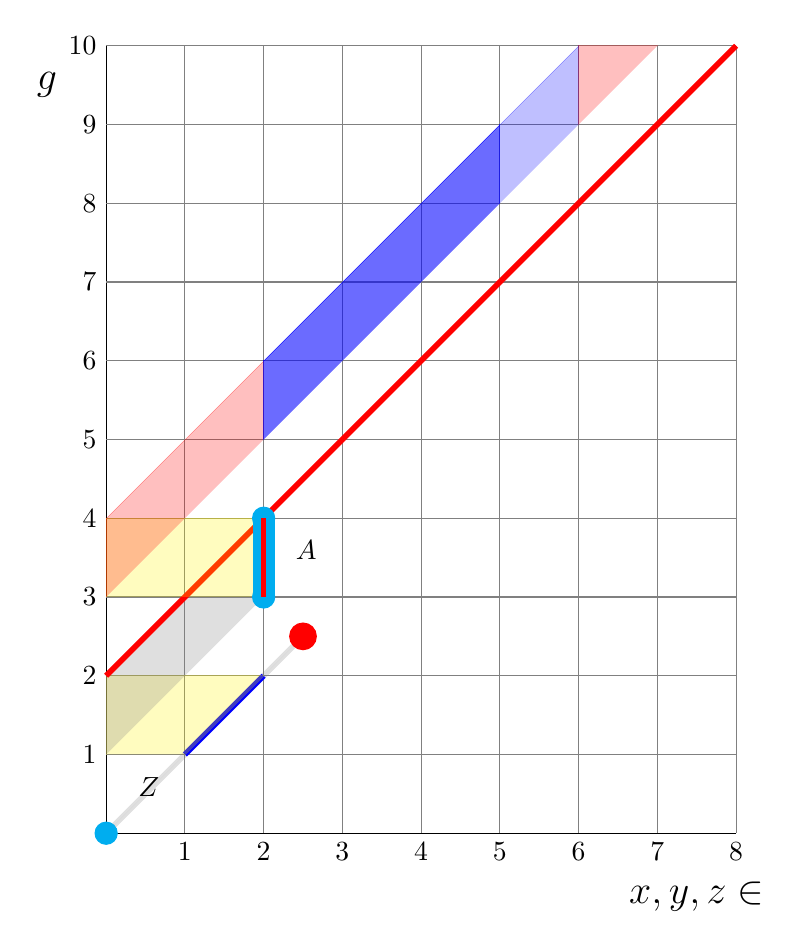
\begin{tikzpicture}
         % grid
         \draw (0,0) -- (8,0);%
         \draw (0,0) -- (0,10);%
         % draw horizontal
         \foreach \y in {1,...,10}%
            {%
               \draw[gray] (0,\y) -- (8,\y);%
               \node[left] at (0,\y) {\y};
            }%
         % draw vertical
         \foreach \x in {1,...,8}%
            {%
               \draw[gray] (\x,0) -- (\x,10);%
               \node[below] at (\x,0) {\x};
            }%

         % complete trace
         \filldraw [gray, opacity = 0.25, line width = 2pt]%
         (0,0) -- (2.5,2.5);%
         \filldraw [blue, opacity = 1, line width = 2pt]% ready
         (2,2) -- (1,1);%
         \filldraw [yellow, opacity = 0.25, line width = 0pt]% reset
         (0,1) -- (0,2) -- (2,2) -- (1,1);%
         \filldraw [gray, opacity = 0.25, line width = 0pt]%
         (0,1) -- (0,2) -- (1,3) -- (2,3);%
         \filldraw [red, opacity = 1, line width = 2pt]% latency
         (0,2) -- (8,10);%

         \filldraw [yellow, opacity = 0.25, line width = 0pt]% reset
         (0,3) -- (0,4) -- (2,4) -- (2,3);%
         \filldraw [red, opacity = 0.25, line width = 0pt]% cancel
         (0,3) -- (0,4) -- (2,6) -- (2,5);%
         \filldraw [blue, opacity = 0.25, line width = 0pt]% done
         (2,5) -- (2,6) -- (5,9) -- (5,8);%
         \filldraw [blue, opacity = 0.25, line width = 0pt]% data
         (2,5) -- (2,6) -- (5,9) -- (5,8);%
         \filldraw [blue, opacity = 0.25, line width = 0pt]% error
         (2,5) -- (2,6) -- (6,10) -- (6,9);%
         \filldraw [red, opacity = 0.25, line width = 0pt]% timeout
         (6,9) -- (6,10) -- (7,10);%

         % def z
         \draw[fill, cyan] (0,0) circle (4pt);
         \node[right] at (0.2, 0.5) {\Large $\mrec\,{{\mreclabel}^{Z}}$};

         % def a
         \draw[fill, cyan] (2,3) circle (4pt);
         \draw[fill, cyan] (2,4) circle (4pt);
         \filldraw [cyan, line width = 8pt] (2,3) -- (2,4);
         \node[right] at (2.2,3.5) {\Large $\mrec\,{{\mreclabel}^{A}}$};

         % send start
         \filldraw [red, opacity = 1, line width = 2pt]% start
         (2,4) -- (2,3);%

         % send close
         \filldraw [red, opacity = 1, line width = 2pt]%
         (2.5,2.5) circle (4pt);

         % axis labels
         \node[below] at (7.5,-0.5) {\Large $x,y,z\in\msetX$};
         \node[left] at (-0.5, 9.5) {\Large $g$};

         % % table of clock values: g
         % \node at (9, 10.5) {\Large $g$};
         % \node at (9, 10) {$10$};
         % \node at (9, 9) {$9$};
         % \node at (9, 8) {$8$};
         % \node at (9, 7) {$7$};
         % \node at (9, 6) {$6$};
         % \node at (9, 5) {$5$};
         % \node at (9, 4) {$4$};
         % \node at (9, 3) {$3$};
         % \node at (9, 2) {$2$};
         % \node at (9, 1) {$1$};
         % \node at (9, 0) {$0$};
         % % table of clock values: x
         % \node at (10, 10.5) {\Large $x$};
         % \node at (10, 10) {$(6,7)$};
         % \node at (10, 9) {$(5,6)$};
         % \node at (10, 8) {$(4,5)$};
         % \node at (10, 7) {$(3,4)$};
         % \node at (10, 6) {$(2,3)$};
         % \node at (10, 5) {$(1,2)$};
         % \node at (10, 4) {$2\mapsto 0$};
         % \node at (10, 3) {$\begin{array}{c}(1,2)\\2\mapsto 0\end{array}$};
         % \node at (10, 2) {$\begin{array}{c}(1,2)\\2\mapsto 0\end{array}$};
         % \node at (10, 1) {$1\mapsto 0$};
         % \node at (10, 0) {$0$};
         % % table of clock values: y
         % \node at (11, 10.5) {\Large $y$};
         % \node at (11, 10) {$10$};
         % \node at (11, 9) {$9$};
         % \node at (11, 8) {$8$};
         % \node at (11, 7) {$7$};
         % \node at (11, 6) {$6$};
         % \node at (11, 5) {$5$};
         % \node at (11, 4) {$4$};
         % \node at (11, 3) {$3$};
         % \node at (11, 2) {$2$};
         % \node at (11, 1) {$1$};
         % \node at (11, 0) {$0$};
      \end{tikzpicture}
   }

   Using the above graph, the following decision diagram can be extracted\TODO[work in progress]:\newline
   % \resizebox{\textwidth}{!}{%
   \resizebox{!}{20cm}{%
      \begin{tikzpicture}[
            every node/.style={xshift=0mm,yshift=0mm,draw,rectangle,rounded corners,fill=gray!20},
            %
            edge from parent/.style={
                  draw,->,
                  nodes={fill=blue!20,rectangle}
               },
            %
            end/.style={
                  nodes={xshift=0mm,yshift=0mm,fill=black,text=white,circle},
                  level distance=20mm
               },
            %
            Zdef/.style={
                  nodes={xshift=0mm,yshift=0mm,fill=green!40,ellipse},
                  edge from parent/.style={
                        midway,draw,->,
                        nodes={fill=green!30,rectangle,xshift=0mm,yshift=0mm}
                     },
                  level distance=30mm
               },
            %
            Zrec/.style={
                  nodes={xshift=0mm,yshift=0mm,fill=green!60,ellipse},
                  edge from parent/.style={
                        midway,draw,->,
                        nodes={fill=green!50,rectangle,xshift=0mm,yshift=0mm}
                     },
                  level distance=35mm
               },
            %
            Adef/.style={
                  nodes={xshift=0mm,yshift=0mm,fill=orange!40,ellipse},
                  edge from parent/.style={
                        midway,draw,->,
                        nodes={fill=orange!30,rectangle,xshift=0mm,yshift=0mm}
                     },
                  level distance=30mm
               },
            %
            Arec/.style={
                  nodes={xshift=0mm,yshift=0mm,fill=orange!60,ellipse},
                  edge from parent/.style={
                        midway,draw,->,
                        nodes={fill=orange!50,rectangle,xshift=0mm,yshift=0mm}
                     },
                  level distance=35mm
               },
            % general actions
            act/.style={
                  nodes={xshift=0mm,yshift=0mm,fill=white,rectangle,rounded corners},
                  edge from parent/.style={
                        draw,->,
                        nodes={fill=cyan!20,rectangle,xshift=0mm,yshift=2mm}
                     },
                  level distance=40mm
               },
            % middle actions in options
            optact/.style={
                  nodes={xshift=0mm,yshift=0mm,fill=white,rectangle,rounded corners},
                  edge from parent/.style={
                        draw,->,
                        nodes={fill=cyan!20,rectangle,xshift=0mm,yshift=0mm}
                     },
                  level distance=45mm
               },
            % always actions
            allact/.style={
                  nodes={xshift=0mm,yshift=0mm,fill=white,rectangle,rounded corners},
                  edge from parent/.style={
                        draw,->,
                        nodes={fill=cyan!20,rectangle,xshift=0mm,yshift=0mm}
                     },
                  level distance=35mm
               },
            % options
            opt/.style={
                  nodes={xshift=0mm,yshift=0mm,fill=magenta!40,diamond},
                  edge from parent/.style={
                        midway,draw,->,
                        nodes={fill=magenta!20,rectangle,xshift=0mm,yshift=0mm}
                     },
                  level distance=48mm
               },
            % nested options
            subopt/.style={
                  nodes={xshift=0mm,yshift=0mm,fill=magenta!40,diamond},
                  edge from parent/.style={
                        midway,draw,->,
                        nodes={fill=magenta!20,rectangle,xshift=0mm,yshift=0mm}
                     },
                  level distance=40mm
               }
         ]
         % root
         \node[act] {$
               \begin{array}{c}
                  g=0 \\% g
                  x=0 \\% x
                  y=0 % y
               \end{array}
            $}
         % def z
         child[Zdef] {
               node {$
                        \begin{array}{c}
                           g=0 \\% g
                           x=0 \\% x
                           y=0 % y
                        \end{array}
                     $}
               % recv ready
               child[act,grow=south west] {
                     node {$
                              \begin{array}{c}
                                 1\leq g\leq 2 \\% g
                                 x=0           \\% x
                                 1\leq y\leq 2 % y
                              \end{array}
                           $}
                     % send latency
                     child[act,grow=south west] {
                           node {$
                                    \begin{array}{c}
                                       2\leq g< 3 \\% g
                                       0\leq x< 2 \\% x
                                       2\leq y< 3 % y
                                    \end{array}
                                 $}
                           % rec z
                           child[Zrec] {
                                 node {$
                                          \begin{array}{c}
                                             g=0 \\% g
                                             x=0 \\% x
                                             y=0 % y
                                          \end{array}
                                       $}
                                 %
                                 edge from parent
                                 node {$
                                          {{\mreclabel}^{Z}}
                                       $}
                              }
                           %
                           edge from parent
                           node[left] {$
                                    \begin{array}{c}
                                       \msend\mathtt{latency}
                                       \\
                                       y-x=2
                                    \end{array}
                                 $}
                        }
                     % send latency or start
                     child[opt,grow=south] {
                           node {$
                                    \begin{array}{c}
                                       3\leq g\leq 4 \\% g
                                       x=2           \\% x
                                       3\leq y\leq 4 % y
                                    \end{array}
                                 $}
                           % send latency
                           child[act,grow=south west]  {
                                 node {$
                                          \begin{array}{c}
                                             3\leq g\leq 4 \\% g
                                             x=2           \\% x
                                             3\leq y\leq 4 % y
                                          \end{array}
                                       $}
                                 % rec z
                                 child[Zrec] {
                                       node {$
                                                \begin{array}{c}
                                                   g=0 \\% g
                                                   x=0 \\% x
                                                   y=0 % y
                                                \end{array}
                                             $}
                                       %
                                       edge from parent
                                       node {$
                                                {{\mreclabel}^{Z}}
                                             $}
                                    }
                                 % label
                                 edge from parent
                                 node[left] {$
                                          \begin{array}{c}
                                             \msend\mathtt{latency}
                                             \\
                                             y-x=2
                                          \end{array}
                                       $}
                              }
                           % send start
                           child[act,grow=south east]  {
                                 node {$
                                          \begin{array}{c}
                                             3\leq g\leq 4 \\% g
                                             x=0           \\% x
                                             3\leq y\leq 4 % y
                                          \end{array}
                                       $}
                                 % def a
                                 child[Adef,grow=south] {
                                       node {$
                                                \begin{array}{c}
                                                   3\leq g\leq 4 \\% g
                                                   x=0           \\% x
                                                   3\leq y\leq 4 % y
                                                \end{array}
                                             $}
                                       % send cancel
                                       child[act,grow=south west] {
                                             node {$
                                                      \begin{array}{c}
                                                         3\leq g\leq 6 \\% g
                                                         0\leq x\leq 2 \\% x
                                                         3\leq y\leq 6 % y
                                                      \end{array}
                                                   $}
                                             % end
                                             child[end] {
                                                   node {$\mend$}
                                                }
                                             %
                                             edge from parent
                                             node[left] {$
                                                      \begin{array}{c}
                                                         \msend\mathtt{cancel}
                                                         \\
                                                         x\leq 2
                                                      \end{array}
                                                   $}
                                          }
                                       % recv done, data or error
                                       child[opt,grow=south] {
                                             node {$
                                                      \begin{array}{c}
                                                         5< g\leq 9 \\% g
                                                         2< x\leq 5 \\% x
                                                         5< g\leq 9 % y
                                                      \end{array}
                                                   $}
                                             % recv done, data or error
                                             child[subopt,grow=south west] {
                                                   node {$
                                                            \begin{array}{c}
                                                               5< g\leq 9 \\% g
                                                               2< x\leq 5 \\% x
                                                               5< g\leq 9 % y
                                                            \end{array}
                                                         $}
                                                   % recv done
                                                   child[optact,grow=south west] {
                                                         node {$
                                                                  \begin{array}{c}
                                                                     5< g\leq 9 \\% g
                                                                     2< x\leq 5 \\% x
                                                                     5< g\leq 9 % y
                                                                  \end{array}
                                                               $}
                                                         % send ok
                                                         child[allact] {
                                                               node {$
                                                                        \begin{array}{c}
                                                                           5< g\leq 9 \\% g
                                                                           2< x\leq 5 \\% x
                                                                           5< g\leq 9 % y
                                                                        \end{array}
                                                                     $}
                                                               % end
                                                               child[end] {
                                                                     node {$\mend$}
                                                                  }
                                                               %
                                                               edge from parent
                                                               node[right] {$\msend\mathtt{ok}$}
                                                            }
                                                         %
                                                         edge from parent
                                                         node[left] {$
                                                                  \begin{array}{c}
                                                                     \mrecv\mathtt{done},
                                                                     \\
                                                                     2<x\leq 5
                                                                  \end{array}$}
                                                      }
                                                   % recv data
                                                   child[optact,grow=south,level distance=45mm] {
                                                         node {$
                                                                  \begin{array}{c}
                                                                     5< g\leq 9 \\% g
                                                                     2< x\leq 5 \\% x
                                                                     5< g\leq 9 % y
                                                                  \end{array}
                                                               $}
                                                         % rec a
                                                         child[Arec] {
                                                               node {$
                                                                        \begin{array}{c}
                                                                           3\leq g\leq 4 \\% g
                                                                           x=0           \\% x
                                                                           3\leq y\leq 4 % y
                                                                        \end{array}
                                                                     $}
                                                               %
                                                               edge from parent
                                                               node {$
                                                                        {{\mreclabel}^{A}}
                                                                     $}
                                                            }
                                                         %
                                                         edge from parent
                                                         node[midway] {$
                                                                  \begin{array}{c}
                                                                     \mrecv\mathtt{data},
                                                                     \\
                                                                     2<x\leq 5
                                                                  \end{array}
                                                               $}
                                                      }
                                                   % recv error
                                                   child[optact,grow=south east] {
                                                         node {$
                                                                  \begin{array}{c}
                                                                     5< g\leq 9 \\% g
                                                                     2< x\leq 5 \\% x
                                                                     5< g\leq 9 % y
                                                                  \end{array}
                                                               $}
                                                         % send restart
                                                         child[allact] {
                                                               node {$
                                                                        \begin{array}{c}
                                                                           5< g\leq 9 \\% g
                                                                           2< x\leq 5 \\% x
                                                                           5< g\leq 9 % y
                                                                        \end{array}
                                                                     $}
                                                               % rec z
                                                               child[Zrec] {
                                                                     node {$
                                                                              \begin{array}{c}
                                                                                 g=0 \\% g
                                                                                 x=0 \\% x
                                                                                 y=0 % y
                                                                              \end{array}
                                                                           $}
                                                                     %
                                                                     edge from parent
                                                                     node {$
                                                                              {{\mreclabel}^{Z}}
                                                                           $}
                                                                  }
                                                               %
                                                               edge from parent
                                                               node[right] {$\msend\mathtt{restart}$}
                                                            }
                                                         %
                                                         edge from parent
                                                         node[right] {$
                                                                  \begin{array}{c}
                                                                     \mrecv\mathtt{error},
                                                                     \\
                                                                     2<x\leq 6
                                                                  \end{array}$}
                                                      }
                                                   %
                                                   edge from parent
                                                   node {$\left\{\mrecv\right\}$}
                                                }
                                             % recv error
                                             child[act,grow=south east] {
                                                   node {$
                                                            \begin{array}{c}
                                                               8< g\leq 10 \\% g
                                                               5< x\leq 6  \\% x
                                                               8< y\leq 10 % y
                                                            \end{array}
                                                         $}
                                                   % send restart
                                                   child[allact] {
                                                         node {$
                                                                  \begin{array}{c}
                                                                     8< g\leq 10 \\% g
                                                                     5< x\leq 6  \\% x
                                                                     8< y\leq 10 % y
                                                                  \end{array}
                                                               $}
                                                         % rec z
                                                         child[Zrec] {
                                                               node {$
                                                                        \begin{array}{c}
                                                                           g=0 \\% g
                                                                           x=0 \\% x
                                                                           y=0 % y
                                                                        \end{array}
                                                                     $}
                                                               %
                                                               edge from parent
                                                               node {$
                                                                        {{\mreclabel}^{Z}}
                                                                     $}
                                                            }
                                                         %
                                                         edge from parent
                                                         node[right] {$\msend\mathtt{restart}$}
                                                      }
                                                   %
                                                   edge from parent
                                                   node[right] {$
                                                            \begin{array}{c}
                                                               \msend\mathtt{error},
                                                               \\
                                                               2<x\leq 6
                                                            \end{array}$}
                                                }
                                             %
                                             edge from parent
                                             node {$\left\{\mrecv\right\}$}
                                          }
                                       % send timeout
                                       child[act,grow=south east] {
                                             node {$
                                                      \begin{array}{c}
                                                         9< g\leq \infty \\% g
                                                         6< x\leq \infty \\% x
                                                         9< y\leq \infty % y
                                                      \end{array}
                                                   $}
                                             % rec z
                                             child[Zrec] {
                                                   node {$
                                                            \begin{array}{c}
                                                               g=0 \\% g
                                                               x=0 \\% x
                                                               y=0 % y
                                                            \end{array}
                                                         $}
                                                   %
                                                   edge from parent
                                                   node {$
                                                            {{\mreclabel}^{Z}}
                                                         $}
                                                }
                                             %
                                             edge from parent
                                             node[right] {$
                                                      \begin{array}{c}
                                                         \msend\mathtt{timeout},
                                                         \\
                                                         6<x
                                                      \end{array}$}
                                          }
                                       %
                                       edge from parent
                                       node {$\mrec\,{{\mreclabel}^{A}}$}
                                    }
                                 edge from parent
                                 node[right] {$
                                          \begin{array}{c}
                                             \msend\mathtt{start},\,x\mapsto 0
                                             \\
                                             x=2
                                          \end{array}
                                       $}
                              }
                           %
                           edge from parent
                           node {$\left\{\msend\right\}$}
                        }
                     % send latency
                     child[act,grow=south east]  {
                           node {$
                                    \begin{array}{c}
                                       4<g\leq\infty \\% g
                                       2<x\leq\infty \\% x
                                       4<y\leq\infty % y
                                    \end{array}
                                 $}
                           % rec z
                           child[Zrec] {
                                 node {$
                                          \begin{array}{c}
                                             g=0 \\% g
                                             x=0 \\% x
                                             y=0 % y
                                          \end{array}
                                       $}
                                 %
                                 edge from parent
                                 node {$
                                          {{\mreclabel}^{Z}}
                                       $}
                              }
                           %
                           edge from parent
                           node[right] {$
                                    \begin{array}{c}
                                       \msend\mathtt{latency}
                                       \\
                                       y-x=2
                                    \end{array}
                                 $}
                        }
                     edge from parent
                     node[left] {$
                              \begin{array}{c}
                                 \mrecv\mathtt{ready},\,x\mapsto 0
                                 \\
                                 1\leq x\leq2
                              \end{array}
                           $}
                  }
               % send close
               child[act,grow=south east] {
                     node {$
                              \begin{array}{c}
                                 g=2.5 \\% g
                                 x=2.5 \\% x
                                 y=2.5 % y
                              \end{array}
                           $}
                     % end
                     child[end] {
                           node {$\mend$}
                        }
                     %
                     edge from parent
                     node[right] {$
                              \begin{array}{c}
                                 \msend\mathtt{close}
                                 \\
                                 x=2.5
                              \end{array}
                           $}
                  }
               %
               edge from parent
               node {$\mrec\,{{\mreclabel}^{Z}}$}
            };
      \end{tikzpicture}
   }
\end{example}


\subsubsection*{Recursion}
The major change is the addition of local clocks \psetX\ to process variables \pvar; allowing, and requiring, that there exists some implementation of local clocks which to be evaluated at run-time.

A subtle change to the definition is the removal of the redundant assignment of a process variable \pvar\ to a continuation process \prc, which is assumed.


\paragraph*{Other approaches}
\TODO[acknowledge other possible approach using affinity]~\cite{Lagaillardie2022}.
\REDO[however, this approach is more formally grounded with respects to the time constraints, ] \TODO